% Options for packages loaded elsewhere
\PassOptionsToPackage{unicode}{hyperref}
\PassOptionsToPackage{hyphens}{url}
\PassOptionsToPackage{dvipsnames,svgnames,x11names}{xcolor}
%
\documentclass[
  20px,
]{article}

\usepackage{amsmath,amssymb}
\usepackage{iftex}
\ifPDFTeX
  \usepackage[T1]{fontenc}
  \usepackage[utf8]{inputenc}
  \usepackage{textcomp} % provide euro and other symbols
\else % if luatex or xetex
  \usepackage{unicode-math}
  \defaultfontfeatures{Scale=MatchLowercase}
  \defaultfontfeatures[\rmfamily]{Ligatures=TeX,Scale=1}
\fi
\usepackage{lmodern}
\ifPDFTeX\else  
    % xetex/luatex font selection
\fi
% Use upquote if available, for straight quotes in verbatim environments
\IfFileExists{upquote.sty}{\usepackage{upquote}}{}
\IfFileExists{microtype.sty}{% use microtype if available
  \usepackage[]{microtype}
  \UseMicrotypeSet[protrusion]{basicmath} % disable protrusion for tt fonts
}{}
\makeatletter
\@ifundefined{KOMAClassName}{% if non-KOMA class
  \IfFileExists{parskip.sty}{%
    \usepackage{parskip}
  }{% else
    \setlength{\parindent}{0pt}
    \setlength{\parskip}{6pt plus 2pt minus 1pt}}
}{% if KOMA class
  \KOMAoptions{parskip=half}}
\makeatother
\usepackage{xcolor}
\usepackage[margin=2cm, paperheight=26cm, paperwidth=50cm]{geometry}
\setlength{\emergencystretch}{3em} % prevent overfull lines
\setcounter{secnumdepth}{5}
% Make \paragraph and \subparagraph free-standing
\makeatletter
\ifx\paragraph\undefined\else
  \let\oldparagraph\paragraph
  \renewcommand{\paragraph}{
    \@ifstar
      \xxxParagraphStar
      \xxxParagraphNoStar
  }
  \newcommand{\xxxParagraphStar}[1]{\oldparagraph*{#1}\mbox{}}
  \newcommand{\xxxParagraphNoStar}[1]{\oldparagraph{#1}\mbox{}}
\fi
\ifx\subparagraph\undefined\else
  \let\oldsubparagraph\subparagraph
  \renewcommand{\subparagraph}{
    \@ifstar
      \xxxSubParagraphStar
      \xxxSubParagraphNoStar
  }
  \newcommand{\xxxSubParagraphStar}[1]{\oldsubparagraph*{#1}\mbox{}}
  \newcommand{\xxxSubParagraphNoStar}[1]{\oldsubparagraph{#1}\mbox{}}
\fi
\makeatother


\providecommand{\tightlist}{%
  \setlength{\itemsep}{0pt}\setlength{\parskip}{0pt}}\usepackage{longtable,booktabs,array}
\usepackage{calc} % for calculating minipage widths
% Correct order of tables after \paragraph or \subparagraph
\usepackage{etoolbox}
\makeatletter
\patchcmd\longtable{\par}{\if@noskipsec\mbox{}\fi\par}{}{}
\makeatother
% Allow footnotes in longtable head/foot
\IfFileExists{footnotehyper.sty}{\usepackage{footnotehyper}}{\usepackage{footnote}}
\makesavenoteenv{longtable}
\usepackage{graphicx}
\makeatletter
\newsavebox\pandoc@box
\newcommand*\pandocbounded[1]{% scales image to fit in text height/width
  \sbox\pandoc@box{#1}%
  \Gscale@div\@tempa{\textheight}{\dimexpr\ht\pandoc@box+\dp\pandoc@box\relax}%
  \Gscale@div\@tempb{\linewidth}{\wd\pandoc@box}%
  \ifdim\@tempb\p@<\@tempa\p@\let\@tempa\@tempb\fi% select the smaller of both
  \ifdim\@tempa\p@<\p@\scalebox{\@tempa}{\usebox\pandoc@box}%
  \else\usebox{\pandoc@box}%
  \fi%
}
% Set default figure placement to htbp
\def\fps@figure{htbp}
\makeatother

\makeatletter
\@ifpackageloaded{caption}{}{\usepackage{caption}}
\AtBeginDocument{%
\ifdefined\contentsname
  \renewcommand*\contentsname{Table of contents}
\else
  \newcommand\contentsname{Table of contents}
\fi
\ifdefined\listfigurename
  \renewcommand*\listfigurename{List of Figures}
\else
  \newcommand\listfigurename{List of Figures}
\fi
\ifdefined\listtablename
  \renewcommand*\listtablename{List of Tables}
\else
  \newcommand\listtablename{List of Tables}
\fi
\ifdefined\figurename
  \renewcommand*\figurename{Figure}
\else
  \newcommand\figurename{Figure}
\fi
\ifdefined\tablename
  \renewcommand*\tablename{Table}
\else
  \newcommand\tablename{Table}
\fi
}
\@ifpackageloaded{float}{}{\usepackage{float}}
\floatstyle{ruled}
\@ifundefined{c@chapter}{\newfloat{codelisting}{h}{lop}}{\newfloat{codelisting}{h}{lop}[chapter]}
\floatname{codelisting}{Listing}
\newcommand*\listoflistings{\listof{codelisting}{List of Listings}}
\makeatother
\makeatletter
\makeatother
\makeatletter
\@ifpackageloaded{caption}{}{\usepackage{caption}}
\@ifpackageloaded{subcaption}{}{\usepackage{subcaption}}
\makeatother

\usepackage{bookmark}

\IfFileExists{xurl.sty}{\usepackage{xurl}}{} % add URL line breaks if available
\urlstyle{same} % disable monospaced font for URLs
\hypersetup{
  pdftitle={TechTraPlastiCE timeline},
  pdfauthor={MdC. Fabio Cruz},
  colorlinks=true,
  linkcolor={blue},
  filecolor={Maroon},
  citecolor={Blue},
  urlcolor={Blue},
  pdfcreator={LaTeX via pandoc}}


\title{TechTraPlastiCE timeline}
\usepackage{etoolbox}
\makeatletter
\providecommand{\subtitle}[1]{% add subtitle to \maketitle
  \apptocmd{\@title}{\par {\large #1 \par}}{}{}
}
\makeatother
\subtitle{External Advisor Commitee: Proposal to Participate}
\author{MdC. Fabio Cruz}
\date{July 30, 2025}

\begin{document}


\section{TechTraPlastiCE Project}\label{techtraplastice-project}

\subsection{Consortium}\label{consortium}

\pandocbounded{
\includegraphics[keepaspectratio]{figures/Consorcio-flags.png}}

🏛️ 9 Higher Education Institutions \textbar{} 1 Association ⏳ Feb.~2025
- Jan.~2028 € 799.887 Euros

\subsection{Main Goal}\label{main-goal}

🎯 The main goal is to \textbf{reinforce the applied research and
technological transfer capacities of the universities} improving their
services portfolios to strengthen the plastic industry's contribution to
the green transition.

🧩🧩 The ambition is to foster the \textbf{collaboration and
partnerships of the University with socio-economic stakeholders} to
incubate, establish and develop circular initiatives, demonstrating
operational success by carrying out joint recycling interventions
integrating actors in the plastics value chain in Colombia, Argentina,
and Chile.

\subsection{Specific Goals}\label{specific-goals}

\begin{itemize}
\item
  SO1: To identify and understand key barriers and leverage points of
  the local plastic companies to generate university-industry
  collaboration opportunities.
\item
  SO2: Create and implement services and solutions portfolios for the
  plastics value chain based on the university's core competencies and
  knowledge.
\item
  SO3: Encourage multi-actor initiatives to enhance the reuse of plastic
  involving waste pickers organizations, companies and the local public
  sectors, taking advantage of the University's articulation capacities.
\item
  SO4: Develop recommendations on new technologies, business models, and
  organizational setups for university-industry collaborations based on
  the lessons learned from the implemented projects as a tool to
  improve, scale up and transfer good practices in HEIs in Latin
  America.
\end{itemize}

\subsection{Approach}\label{approach}

\pandocbounded{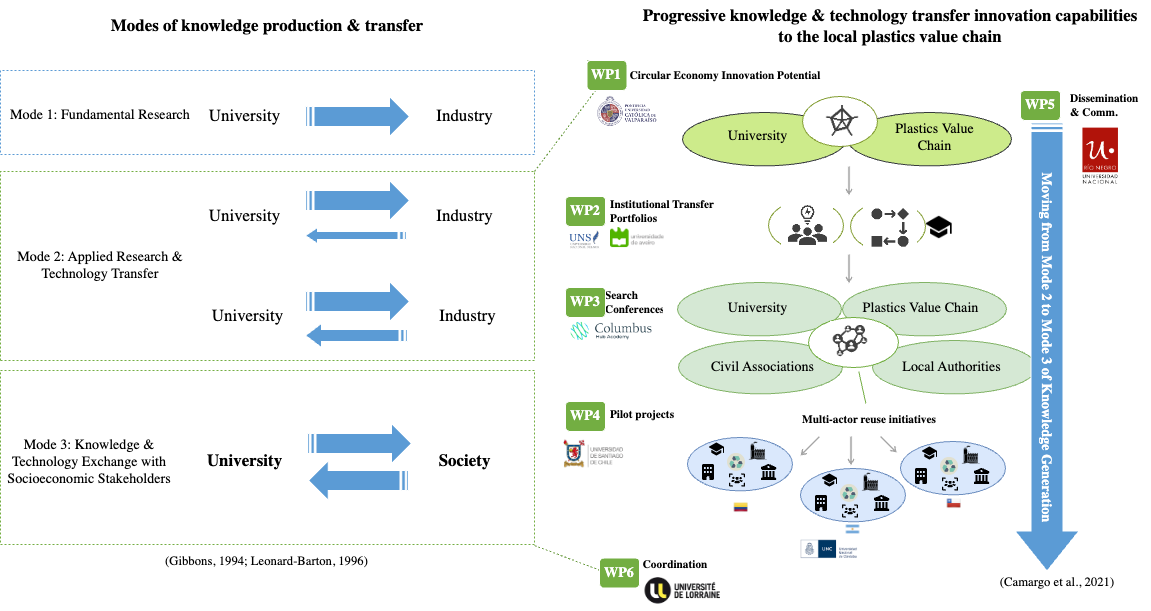
\includegraphics[keepaspectratio]{figures/TechTraPlastiCE-Approach.png}}

\subsection{Milestones}\label{milestones}

\pandocbounded{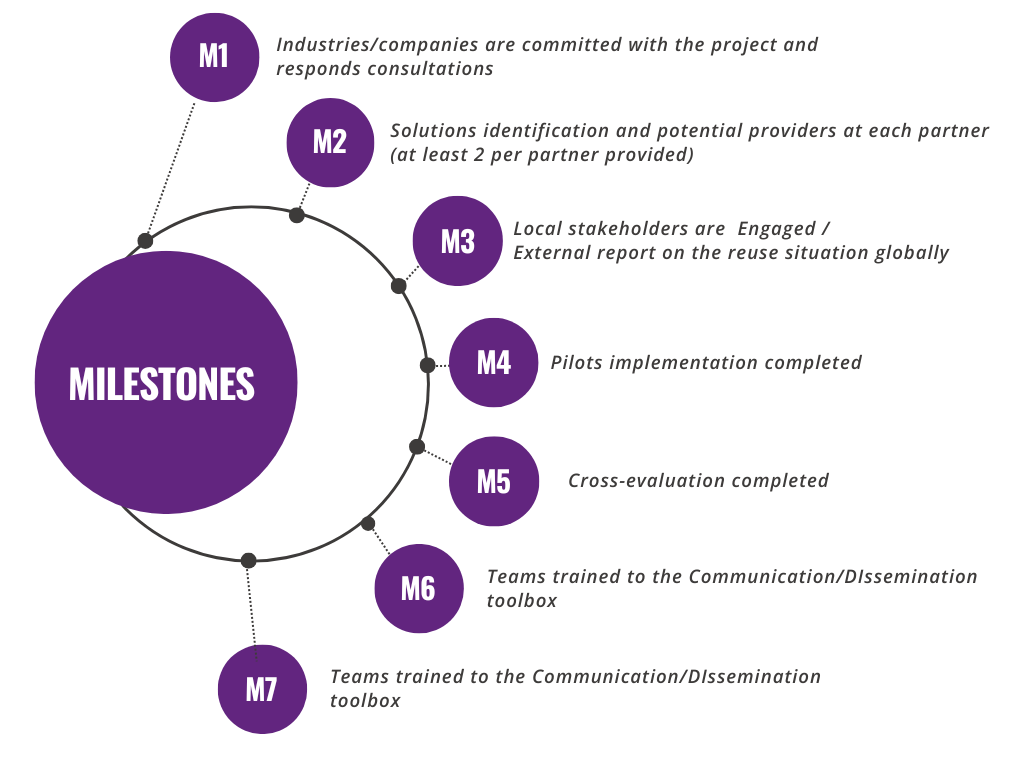
\includegraphics[keepaspectratio]{figures/Milestones.png}}

\section{External Advisory Board}\label{external-advisory-board}

\textbf{Objective}:

\begin{quote}
The main objective of the EAB is \textbf{to provide independent,
strategic advice} to the project consortium based on the intermediary
results, thereby enhancing the overall scientific and societal impact of
the initiative.
\end{quote}

\subsection{Work Plan}\label{work-plan}

The work plan will consist in the following elements;

\begin{ganttchart}[vgrid,
   y unit title=0.5cm,
   y unit chart=0.5cm,
   x unit = 0.7cm,
   time slot format=isodate-year,
   time slot unit=month,
   today=2025-07,
   progress=today,
   title/.append style={draw=none, fill= Neutro},
   title label font=\sffamily\bfseries\color{white},
   title label node/.append style={below=-1.6ex},
   title left shift=.05,
   title right shift=-.05,
   title height=1,
   bar/.append style={draw=none, fill=OliveGreen!75},
   bar height=.6,
   bar label font=\normalsize\color{black!50},
   group right shift=0,
   group top shift=.6,
   group height=.3,
   group peaks height=.2,
   bar incomplete/.append style={fill=Celeste},
   bar progress label anchor = west,
   bar progress label font = \color{white}\scriptsize
]{2025-02}{2028-01}

\gantttitle[]{TechTraPlastiCE timeline}{36}\\  
\gantttitlecalendar{year} \\
\gantttitlelist{"Q1","Q2","Q3","Q4", "Q1","Q2","Q3","Q4","Q1","Q2","Q3","Q4"}{3}\\ % Semester title
\gantttitlecalendar{month} \\



% Working package 1
\ganttgroup{WP 1: Innovation Opportunities for Circular Economy}{2025-02}{2025-10} \\

% Tareas
\ganttbar[name=1a, progress=100, progress label text={Completed}]{Developing a framework to understand the companies/industries' performance for circular economy}{2025-02}{2025-04} \\
\ganttbar[name=1b, progress=80, progress label text={90\%}]{Identifying gaps and drivers at targeted Industries/Companies to comply with the norms and consumers' preferences}{2025-05}{2025-10} \\
\ganttbar[name=1c, progress=10, progress label text={10\%}]{Assessing the innovation capacities of the industries/sectors}{2025-05}{2025-10} 
\ganttnewline[thick, blue]  \\
\ganttmilestone[]{Milestone 1}{2025-04} \\


% Working package 2
\ganttgroup{WP2: Development of a networked portfolio}{2025-07}{2026-04} \\

% Tareas
\ganttbar[name=2a, progress=0, progress label text={ }]{Identifying existing core services for plastics challenges within the network of partners}{2025-07}{2026-01} \\
\ganttbar[name=2b, progress=0,  progress label text={ }]{Design of Institutional Portfolios}{2025-11}{2026-04} \\
\ganttbar[name=2c, progress=0,  progress label text={ }]{Promoting cross-peer collaboration and mentoring}{2025-11}{2026-04} 
\ganttnewline[thick, blue] 
\\


% Working package 3
\ganttgroup{WP3: Multi-actor collaborations for just and safe plastic’s circular economy }{2026-02}{2027-04} \\

% Tareas
\ganttbar[name=3a, progress=0, progress label text={ }]{Reuse action clues in Argentina, Chile and Colombia}{2026-02}{2026-04} \\
\ganttbar[name=3b, progress=0,  progress label text={ }]{Engaging local stakeholders}{2026-02}{2026-10} \\
\ganttbar[name=3c, progress=0,  progress label text={ }]{Assessment of local reuse systems and benchmarking with impactful reuse practices}{2026-05}{2026-10} \\
\ganttbar[name=3d, progress=0,  progress label text={ }]{Search Conference}{2026-08}{2027-04} \\
\ganttbar[name=3e, progress=0,  progress label text={ }]{Implementation of collaborative initiatives}{2026-11}{2027-04} \\


% Working package 4
\ganttgroup{WP3: Pilot projects implementation}{2026-02}{2027-04} \\

% Tareas
\ganttbar[name=4a, progress=0, progress label text={ }]{Pedagogical Integration of Industry at the University}{2026-02}{2026-04} \\
\ganttbar[name=4b, progress=0,  progress label text={ }]{Pilots implementation}{2026-02}{2026-10} \\
\ganttbar[name=4c, progress=0,  progress label text={ }]{Cross evaluation of pilot projects between Latin American Universities}{2026-05}{2026-10} \\
\ganttbar[name=4d, progress=0,  progress label text={ }]{Institutional Recommendations}{2026-08}{2027-04} \\

% Working package 5
\ganttgroup{WP5: Communication and Dissemination}{2025-02}{2028-01} \\

% Tareas
\ganttbar[name=5a, progress=0, progress label text={ }]{Definition of a dissemination strategy and its implementation.}{2025-02}{2026-05} \\
\ganttbar[name=5b, progress=0,  progress label text={ }]{Dissemination Toolbox and Training}{2025-02}{2026-8} \\
\ganttbar[name=5c, progress=0,  progress label text={ }]{Project Website Launching and Monitoring}{2025-05}{2028-01} \\
\ganttbar[name=5d, progress=0,  progress label text={ }]{Establishing an Open Digital Repository}{2026-08}{2027-04} \\
\ganttbar[name=5e, progress=0,  progress label text={ }]{Final Conference}{2027-01}{2028-01} \\


% Working package 6
\ganttgroup{WP6: Project management and Quality assurance}{2025-02}{2028-01}\\

% Tareas
\ganttbar[name=6a, progress=0, progress label text={ }]{Partnership agreement management with the consortium}{2025-02}{2025-05} \\
\ganttbar[name=6b, progress=0,  progress label text={ }]{Financial management guidelines, monitoring and reports}{2025-02}{2028-01} \\
\ganttbar[name=6c, progress=0,  progress label text={ }]{Project Management guidelines, monitoring and reports}{2025-02}{2028-01} \\
\ganttbar[name=6d, progress=0,  progress label text={ }]{Establishment of quality guidelines and an external committee for monitoring the advancement of the project}{2025-02}{2028-01} \\
\ganttbar[name=6e, progress=0,  progress label text={ }]{Organization of the Kick-off meeting at Nancy}{2025-02}{2025-05} \\


\ganttset{link/.style={Naranja}}

% WP1   
\ganttlink{1a}{1b}
\ganttlink{1a}{1c}

\ganttlink{1b}{3c}
\ganttlink{1c}{3c}

% WP2   
\ganttlink{2a}{2b}
\ganttlink{2b}{2c}

\ganttlink{2a}{3c}

% WP3
\ganttlink{3a}{3b}
\ganttlink{2b}{2c}
\ganttlink{2b}{2c}


%\ganttlink{1b}{}
%\ganttlink{T1.1}{T1.4}
%\ganttlink{T1.1}{T1.5}
%\ganttlink{T1.4}{Mile1}

         


\end{ganttchart}

\subsection{Composition}\label{composition}

The major requirements are

\begin{enumerate}
\def\labelenumi{\arabic{enumi}.}
\tightlist
\item
\item
\item
\end{enumerate}

\subsubsection{Maria José Zapata}\label{maria-josuxe9-zapata}

\begin{figure}

\begin{minipage}{0.30\linewidth}

\begin{figure}[H]

{\centering \pandocbounded{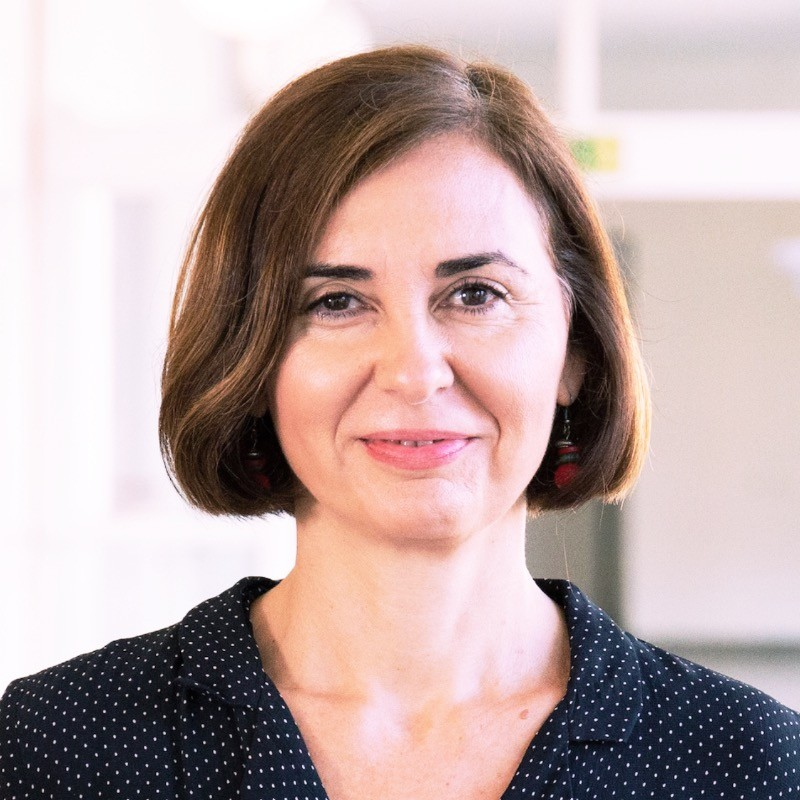
\includegraphics[keepaspectratio]{figures/Maria-Jose.jpeg}}

}

\end{figure}%

\end{minipage}%

\end{figure}%

\subsubsection{Ferran GIones}\label{ferran-giones}

\begin{figure}

\begin{minipage}{0.30\linewidth}

\begin{figure}[H]

{\centering \pandocbounded{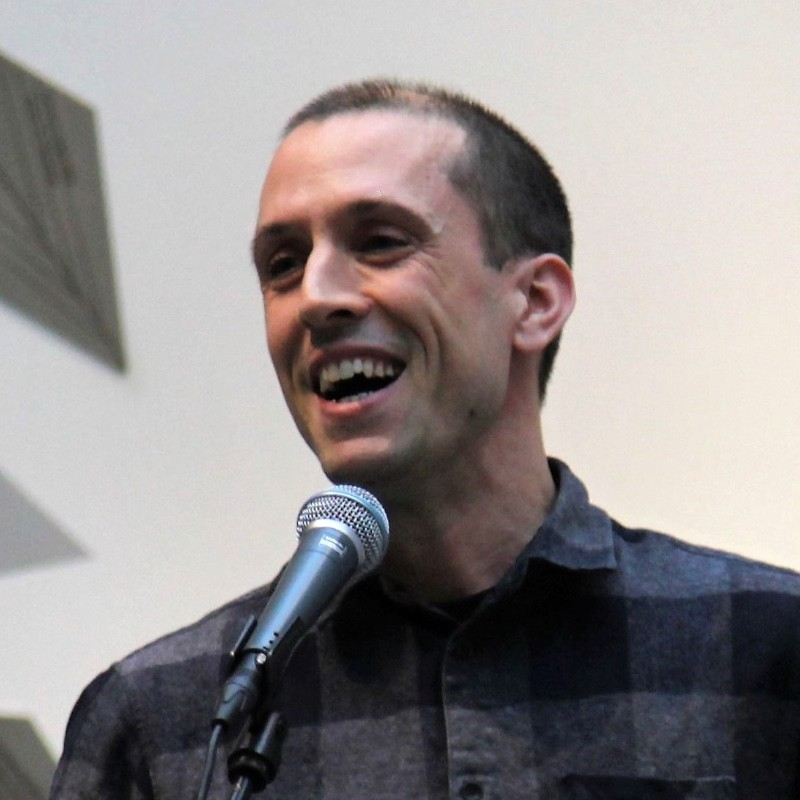
\includegraphics[keepaspectratio]{figures/Ferran-Giones.jpg}}

}

\end{figure}%

\end{minipage}%

\end{figure}%

\subsubsection{Astrid}\label{astrid}




\end{document}
